\chapter{Autómatas Finitos y Gramáticas Regulares}

\textbf{Teorema: }La clase de los lenguajes generados por una gramática regular es precisamente la de los lenguajes regulares.

\section{Procedimiento de Conversión de una GR a un AF}
\begin{enumerate}
\item Para cada símbolo no terminal de la gramática asociar un estado en el autómata.
\item Para cada regla $A::=bC$ en la gramática origina una transición $(A,b,C)$ en el autómata.
\item Para cada regla $A::=b$ se tendrá transiciones $(A,b,Z)$ donde $Z$ será el único estado final del autómata.
\end{enumerate}

\textbf{Ejemplo: }Sea la GR $G=(\Sigma_N,\Sigma_T,S,P)$ donde $P$ esta dado por:
\begin{align*}
\mbox{Del ejemplo anterior: }	\\
S::=aA	\\
S::=bA	\\
A
\end{align*}
%grafico 14.1
\begin{figure}[h!]
\centering
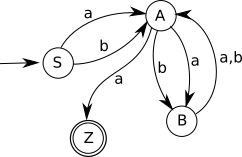
\includegraphics[width=0.4\textwidth]{img_14_1.png}
\caption{Diagrama de Transición}\label{img_14_1}
\end{figure}

\section{Procedimiento de Conversión de un AFD a un GR}

\begin{enumerate}
\item Para cada transición de la forma $((\downlegend{p}{(1)},a),\downlegend{q}{(2)})$ en el AFD( (1): estado anterior, (2): estado siguiente), donde:

$p,q\in S, a\in I$ habrá una regla $X_p::=aX_q$ en la gramática. En la que $X_i$ es la variable en que corresponde al estado $i$ del AFD.
\item Para cada transición $((p,a),q)$ donde $q\in F$ incorpora ademas la regla.
$$X_p::=a\qquad (\mbox{también }X_p::=aX_q)$$
\end{enumerate}
\textbf{Ejemplo: }Dado el AFD. Obtener la GR equivalente.
%grafico 14.2
\begin{figure}[h!]
\centering
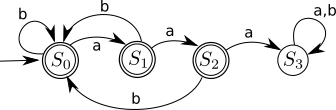
\includegraphics[width=0.4\textwidth]{img_14_2.png}
\caption{Diagrama de Transición}\label{img_14_2}
\end{figure}

\textbf{Solución: }Se obtiene las siguientes reglas:
\begin{align*}
P\left \{ \begin{array}{c}
s_0::=bs_0	\\
s_0::=as_1	\\
s_1::=as_2	\\
s_1::=bs_0	\\
s_2::=as_3	\\
s_2::=as_0	\\
s_3::=as_3	\\
s_3::=bs_3	\\
s_0::=b	\\
s_0::=a	\\
s_1::=a	\\
s_1::=b	\\
s_2::=b
\end{array}\right.
\end{align*}
Dado un AFD $D=(S,I,\delta,s^*,F)$ se desea encontrar un GLD $G$, tal que $L(D)=L(G)$. Si $q$ no es un estado final, la gramática buscada es $G=(\Sigma_N,\Sigma_T,P,q)$ en la que $P$ consiste de reglas de la forma: 
\begin{align*}
p&::=aq	&\mbox{Si }\delta(p,a)=q	\\
p&::=a	&\mbox{Si }\delta(p,a)=q\in F
\end{align*}
\textbf{Ejemplo: }Sea el AFD $D$ dado por Fig \ref{img_14_3}:
%grafico 14.3
\begin{figure}[h!]
\centering
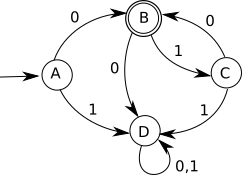
\includegraphics[width=0.4\textwidth]{img_14_3.png}
\caption{Diagrama de Transición}\label{img_14_3}
\end{figure}
\begin{align*}
A&::=0B	\\
A&::=1D\qquad\xmark	\\
B&::=0D\qquad\xmark	\\
B&::=1C	\\
C&::=0B	\\
C&::=1D\qquad\xmark	\\
D&::=0D\qquad\xmark	\\
D&::=1D\qquad\xmark	\\
A&::=0	\\
C&::=0
\end{align*}
$D$ es un estado muerto, quitamos las reglas de la forma $p::aD$

Quedará:
\begin{align*}
P\left \{ \begin{array}{c}
A::=0B	\\
B::=1C	\\
C::=0B	\\
A::=0	\\
C::=0
\end{array}\right.
\end{align*}
$0$ y $1$ son $\Sigma_T$

\section{Conversión de una Gramática Regular GR a AFND-$\varepsilon$}
Sea la GLD $G=(\Sigma_N,\Sigma_T,s,P)$ encontraremos un AFND-$\varepsilon$.
$$N=(S^{nd},I^{nd},\delta^{nd},s^*,F^{nd})$$
tal que $L(G)=L(N)$

Sea:
\begin{enumerate}
\item $I^{nd}=\Sigma_T$
\item Los estados $S^{nd}$ de $N$ serán $S$ además de los sufijos de la parte derecha de las reglas.
\item $s^*=S$
\item Para definir $\delta$, se tiene:
	\begin{itemize}
	\item Si $\alpha::=\beta\quad\in P$ entonces se define $\delta(\alpha,\varepsilon)=\beta$
	\item Si $a\alpha\in S^{nd},a\in I^{nd}$ se hace $\delta(a\alpha,a)=\alpha$
	\end{itemize}
\end{enumerate}
Los estados finales $F^{nd}$ del autómata $N$ serán los estados rotulados como $\varepsilon$.

\textbf{Ejemplo: }Sea $G$ la GLD definida por:
\begin{align*}
\Sigma_T&=\{0,1\}	\\
S&::=0A	\\
A&::=|A|\varepsilon
\end{align*}
Obtener el AF equivalente.

\textbf{Solución: }
\begin{itemize}
\item $I^{nd}=\{0,1\}\cup\{\varepsilon\}$
\item $S^{nd}=\{S,0A,1A,\uplegend{A}{sufijo},\varepsilon\}$
\item $s^*=S$
\item Diagrama en Fig \ref{img_14_4}.
%grafico 14.4
\begin{figure}[h!]
\centering
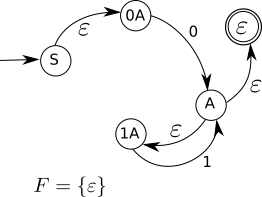
\includegraphics[width=0.4\textwidth]{img_14_4.png}
\caption{Diagrama de Transición}\label{img_14_4}
\end{figure}

\end{itemize}
\section{Jerarquía de las Gramáticas}
De acuerdo a Noam Chomsky se tiene la siguiente clasificación para las gramáticas.
\begin{enumerate}
\item G. Regulares.
\item G. Sensibles al contexto.
\item G. sin Restricciones.
\item G. Libres de contexto.
\end{enumerate}
\section{Gramáticas Sensibles al Contexto}
También se les conoce como gramáticas del tipo I y sus producciones son de la forma.
\begin{align*}
&xAy\rightarrow xvy&\\
A\in\Sigma_N,&\quad x,y\in\Sigma^*,&\quad v\in\Sigma^*
\end{align*}
En una gramática S. Contexto no hay reglas compresoras.

\textbf{Ejemplo: }Sea G la gramática.
\begin{align*}
S::=&\overbrace{abc}^{R_1}|\overbrace{aAbc}^{R_2}	\\
A::=&\overbrace{abc}^{R_3}|\overbrace{aAbc}^{R_4}	\\
Cb::=&\overbrace{bC}^{R_5}	\\
Cc::=&\overbrace{cc}^{R_6}
\end{align*}

\begin{align*}
S	&::=aAbc	&(R_2)	\\
	&::=aabCbc	&(R_3)	\\
	&::=aabbCc	&(R_5)	\\
	&::=aabbccc	&(R_6)	\\
\end{align*}

$L(G)=\{abc,\overbrace{aa}^{a^2}\overbrace{bb}^{b^2}\overbrace{ccc}^{c^3}, a^3b^3c^3,...\}$

$L(G)=\{a^nb^nc^n/n\geq 1\}$

\section{G. Sin Restricciones}
Se llaman también recursivamente enumeradas o gramáticas del tipo ''O''. Sus reglas son de la forma:

$xAy::=v\qquad A\in\Sigma_N;x,y,v\in\Sigma^*	$

\textbf{Ejemplo: }La gramática G:
\begin{align*}
\left \{ \begin{array}{c}
aS::=bSb	\\
aSb::=\varepsilon	\\
SbS::=bcS
\end{array}\right.
\end{align*}
Es una gramática sin restricciones.

\section{G. Libres de Contexto}
También conocidos como gramáticas del tipo 2. Se caracterizan porque la parte izquierda de la regla está formado por un único símbolo no terminal.
$$A::=v;	\qquad A\in\Sigma_N; \qquad v\in\Sigma^*=\Sigma_N\cup\Sigma_T;\cup:  combinacion$$

Estas gramáticas son especialmente adecuadas para representar los aspectos sintácticos de un lenguaje de programación. Se observa de la definición que podemos incluir $A\rightarrow\varepsilon$.

\textbf{Ejemplo: }
\begin{enumerate}
\item Sea $\Sigma_T=\{a,b\}$ y $P$.
\begin{align*}
S::=\overbrace{\varepsilon}^{R_1}|\overbrace{aSb}^{R_2}	\\
S::=aSb\qquad(R_2)	\\
S::aaSbb\qquad(R_2)	\\
S::=aaaSbbb\qquad(R_2)	\\
S::=a^nSb^n\qquad(R_2)	\\
S::=a^n\varepsilon b^n=a^nb^n\qquad(R_1)	\\
L(G)=\{a^nb^n/n\geq 0\}	\\
\mbox{ya que }	\\
S::=\varepsilon	\\
S\rightarrow\varepsilon
\end{align*}
\item Sea $\Sigma_T=\{a,b\}$ y $P$.
$$S::=\underbrace{aSa}_{R_1}|\underbrace{bSb}_{R_2}|\underbrace{a}_{R_3}|\underbrace{a}_{R_4}|\underbrace{\varepsilon}_{R_5}$$
\begin{align*}
L=\{a,b,\varepsilon,abaaaaba,...\}	\\
S::=aba\qquad(R_1)	\\
S::=abSba\qquad(R_2)	\\
S::=abaSaba\qquad(R_1)	\\
S::=abaaSaaba\qquad(R_2)	\\
S::=abaa|aaba\qquad(R_5)	\\
L=\{uu^R/u\in\Sigma^*\}	\\
L=\{w/w=w^R,w\in\Sigma^*\}
\end{align*}
\item Sea $\Sigma=\{a,b\}$ y $P$ dado por:
\begin{align*}
S::=aS|aB	\\
B::=bC	\\
B::=bC	\\
c::=aC|a
\end{align*}
\end{enumerate}